\chapter{Editor umožňujúci konkurentné úpravy jedného dokumentu}

\label{kap:zdialtelnost} % id kapitoly pre prikaz ref

Myšlienka kolaboratývneho editora bola prvýkrát zaznamenaná už v roku 1968 Douglas Engelbart-om. 
Avšak do popularity sa dostala až nedávno, približne 20 rokov od prvého záznamu.
Kolaboratívny editor umožnuje viacerým užívaťeľom upravovať jeden dokument.
Tieto editory sa rozďeľujú na dve kategórie
\begin{itemize}
  \item Real time - zmeny dokumentu sa okamžite zobrazia všetkým používateľom
  \item Non-real-time - zmeny dokumentu sa nedejú okamžite (podobne ako pri verzionovacých
  systémoch ako Git, Mercurial)
\end{itemize}
My sa v práci zameriavame real time editormi, kde je treba riešiť synchronizáciu editorových
inštancii používateľov a riešenie možných konfliktov.

\section{Real time kolaboratívnt editor}
Problematika real time kolaboratívnych editorov sa dá rozdeliť do samostatných zmysluplných 
podkapitol
\begin{itemize}
\item  technické výzvy
\item  algoritmy riešiace konkurentné modifikácie jedného zdroja
\item  súčasný stav riešenej problematiky doma a v zahraničí,
\item  cieľ práce,
\item  metodika práce a metódy skúmania,
\item  výsledky práce, 
\end{itemize}

\subsection{Technické výzvy}
Technické vźyvy pramenia z asynchrónnej komunikácie po sieti. Teoreticky, keby táto 
komnikácia bola instantná, tak vytvorenie takéhoto editora, by nebolo priveľmi odlišné od
editora pre jedného používateľa. Algoritmus, rišiaci takýto problém by mohol fungovať na 
základe \textit{upravovacieho zámku}. Fungoval by celkom jednoducho:
\begin{enumerate}
  \item Požiadanie servera o \textit{upravovacý zámok}
  \item Počkanie na schválenie zo servera, že sme na rade s úpravou
  \item Úprava dokumentu
  \item Vzdanie sa \textit{upravovacieho zámku}
\end{enumerate}
Avšak rýchlosť komunikácie je obmedzená latenciou siete. To vytvára základnú dilemu: 
užívatelia potrebujú okamžite vlastné úpravy, ktoré sú do dokumentu zapracované,
ale ak sú začlenené okamžite, potom kvôli latencii komunikácie musia byť ich
úpravy nevyhnutne vložené do rôznych verzií dokumentu.

Výzvou v spolupráci v reálnom čase je teda presne zistiť, ako možno aplikovať úpravy
od vzdialených používateľov, ktoré boli pôvodne vytvorené vo verziách dokumentu, ktor
nikdy neexistovali na mieste a ktoré môžu byť v rozpore s vlastnými 
miestnymi úpravami používateľa.

Najsofistikovanejšie riešenia vyriešia tento problém spôsobom, ktorý nevyžaduje server,
nepoužíva uzamknutie (všetci používatelia môžu voľne upravovať všetky časti dokumentu súčasne) 
a podporuje ľubovoľný počet používateľov (obmedzený iba zdrojmi počítačov). 
UNA a SubEthaEdit sú príklady dvoch programov, ktoré využívajú tento prístup.
Tieto programy sú však dostupné iba pre operačných systémoch macOS a využívajú technológie,
ako napríklad \cite{bonjour},ktoré sú špecifické pre tento OS.

Zatiaľ čo tieto sofistikované prístupy umožňujú najlepšiu používateľskú skúsenosť,
v klientskom serveri môže byť vytvorený aj základný editor pre spoluprácu. Pri scenári
klient-server je pri otvorení dokumentu priradená jedna z inštancií editora úloha servera
spolupráce. Tento server zaisťuje, že ostatné editory sú synchronizované určovaním
latencie siete a fungovaním ako server synchronizácie času. Server obdrží upozornenia
na časové označenie zmien vykonaných v dokumente inými používateľmi. 
Určuje, ako majú tieto zmeny ovplyvňovať svoju lokálnu kópiu, a vysiela jej zmeny do
fondu spolupráce. V niektorých modeloch sa zmeny na klienta neodzrkadľujú dovtedy,
kým sa zo servera nevráti oficiálna odpoveď, a to aj vtedy, ak boli tieto zmeny vykonané lokálne.
Príkladom takéhoto editora je napríklad Gobby.

My sme sa v práci rozhodli použiť klient-server model, pričom za synchronizáciu klientov
je zodpovedný výhradne server. Podobný prístup používa napr. spoločnost Google v produktoch
ako Google dokumenty a tabuľky.

\subsection{Algoritmy riešiace konkurentné modifikácie}
Na riešenie synchronizácie klientov existujú dva dobre preskúmané typy algoritmov.
\begin{enumerate}
  \item OT - Prevádzková transformácia (Operational transformation)
  \item CRDT - Bezkonfliktné idempotentné dátové typy (Conflict-free replicated data type)
\end{enumerate}
V práci použijeme CRDT, pretože OT je predchodca CRDT a v praxi často nefunguje tak dobre,
ako to autori zamýšľali. Taktiež použitie OT je komplikované a neškálovateľné \cite{ot_nonscalable}.

\begin{flushleft}\textbf {CRDT}\end{flushleft}
Problém súbežnej modifikácie jedného textového poľa je, že jednoduché operácie ako
pridaj písmeno a zmaž písmneo, nie sú komutatívne. Keďže používatelia modifikujú dokument
cez sieť, nemáme zaručené v akom poradí sa modifikácie uskutočnia. Ilustrujme tento
problém na príklade:

\begin{figure}
\centerline{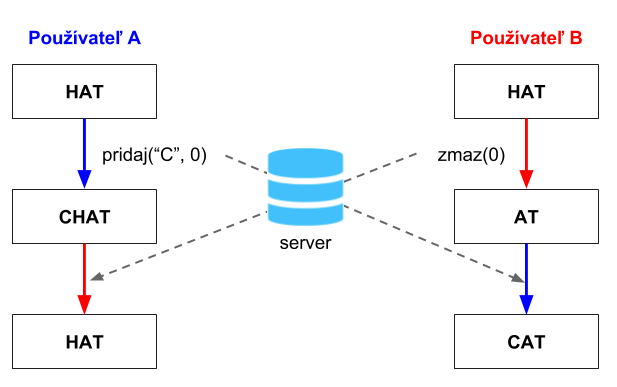
\includegraphics[width=0.8\textwidth]{images/nekomutativne_operacie}}
%popis obrazku
\caption[Nekomutativita textových operácii]{Nekomutativita textových operácii}
%id obrazku, pomocou ktoreho sa budeme na obrazok odvolavat
\label{obr:cursus}
\end{figure}

TODO: nieco o tom ako ako CRDT funguje

\subsection{Súčasný stav}
V časti súčasný stav riešenej problematiky doma a v zahraničí autor uvádza 
dostupné informácie a poznatky týkajúce sa danej témy. Zdrojom pre spracovanie sú 
aktuálne publikované práce domácich a zahraničných autorov.  Podiel tejto časti práce 
má tvoriť približne 30 \% práce.

\subsection{Cieľ práce}
Časť cieľ práce  školského diela jasne, výstižne a presne charakterizuje predmet 
riešenia. Súčasťou sú aj rozpracované čiastkové ciele, ktoré podmieňujú dosiahnutie 
cieľa hlavného. 

\subsection{Metodika práce a metódy skúmania}
Časť metodika práce a metódy skúmania spravidla obsahuje:
\begin{enumerate}
\item  charakteristiku objektu skúmania,  
\item  pracovné postupy, 
\item  spôsob získavania údajov a ich zdroje, 
\item  použité metódy vyhodnotenia a interpretácie výsledkov,
\item  štatistické metódy.
\end{enumerate}

\subsection{Výsledky práce a diskusia}
Časti výsledky práce a diskusia sú najvýznamnejšími  časťami  školského diela. 
Výsledky (vlastné postoje alebo vlastné riešenia), ku ktorým autor dospel, sa musia 
logicky usporiadať a pri opisovaní sa musia dostatočne zhodnotiť. Zároveň sa 
komentujú všetky skutočnosti a poznatky v konfrontácii s výsledkami iných autorov. 
Výsledky práce a diskusia môžu tvoriť aj jednu samostatnú časť  a spoločne tvoria 
spravidla 30 až 40 \% školského diela.  
